%%%%%%%%%%%%%%%%%%%%%%%%%%%%%%%%%%%%%%%%%
% Structured General Purpose Assignment
% LaTeX Template
%
% This template has been downloaded from:
% http://www.latextemplates.com
%
% Original author:
% Ted Pavlic (http://www.tedpavlic.com)
%
% Note:
% The \lipsum[#] commands throughout this template generate dummy text
% to fill the template out. These commands should all be removed when 
% writing assignment content.
%
%%%%%%%%%%%%%%%%%%%%%%%%%%%%%%%%%%%%%%%%%

%----------------------------------------------------------------------------------------
%	PACKAGES AND OTHER DOCUMENT CONFIGURATIONS
%----------------------------------------------------------------------------------------

\documentclass{article}

\usepackage{fancyhdr} % Required for custom headers
\usepackage{lastpage} % Required to determine the last page for the footer
\usepackage{extramarks} % Required for headers and footers
\usepackage{graphicx} % Required to insert images
\usepackage{caption}
\usepackage{float}
\usepackage{url}
\usepackage{subcaption}


% Margins
\topmargin=-0.45in
\evensidemargin=0in
\oddsidemargin=0in
\textwidth=6.5in
\textheight=9.0in
\headsep=0.25in 


\linespread{1.1} % Line spacing

% Set up the header and footer
\pagestyle{fancy}
\lhead{\hmwkAuthorName} % Top left header
\chead{\hmwkClass\ \hmwkTitle} % Top center header
\rhead{\firstxmark} % Top right header
\lfoot{\lastxmark} % Bottom left footer
\cfoot{} % Bottom center footer
\rfoot{Page\ \thepage\ of\ \pageref{LastPage}} % Bottom right footer
\renewcommand\headrulewidth{0.4pt} % Size of the header rule
\renewcommand\footrulewidth{0.4pt} % Size of the footer rule

\setlength\parindent{0pt} % Removes all indentation from paragraphs

%----------------------------------------------------------------------------------------
%	DOCUMENT STRUCTURE COMMANDS
%	Skip this unless you know what you're doing
%----------------------------------------------------------------------------------------

% Header and footer for when a page split occurs within a problem environment
\newcommand{\enterProblemHeader}[1]{
\nobreak\extramarks{#1}{#1 continued on next page\ldots}\nobreak
\nobreak\extramarks{#1 (continued)}{#1 continued on next page\ldots}\nobreak
}

% Header and footer for when a page split occurs between problem environments
\newcommand{\exitProblemHeader}[1]{
\nobreak\extramarks{#1 (continued)}{#1 continued on next page\ldots}\nobreak
\nobreak\extramarks{#1}{}\nobreak
}

\setcounter{secnumdepth}{0} % Removes default section numbers
\newcounter{homeworkProblemCounter} % Creates a counter to keep track of the number of problems

\newcommand{\homeworkProblemName}{}
\newenvironment{homeworkProblem}[1][Problem \arabic{homeworkProblemCounter}]{ % Makes a new environment called homeworkProblem which takes 1 argument (custom name) but the default is "Problem #"
\stepcounter{homeworkProblemCounter} % Increase counter for number of problems
\renewcommand{\homeworkProblemName}{#1} % Assign \homeworkProblemName the name of the problem
\section{\homeworkProblemName} % Make a section in the document with the custom problem count
\enterProblemHeader{\homeworkProblemName} % Header and footer within the environment
}{
\exitProblemHeader{\homeworkProblemName} % Header and footer after the environment
}

\newcommand{\problemAnswer}[1]{ % Defines the problem answer command with the content as the only argument
\noindent\framebox[\columnwidth][c]{\begin{minipage}{0.98\columnwidth}#1\end{minipage}} % Makes the box around the problem answer and puts the content inside
}

\newcommand{\homeworkSectionName}{}
\newenvironment{homeworkSection}[1]{ % New environment for sections within homework problems, takes 1 argument - the name of the section
\renewcommand{\homeworkSectionName}{#1} % Assign \homeworkSectionName to the name of the section from the environment argument
\subsection{\homeworkSectionName} % Make a subsection with the custom name of the subsection
\enterProblemHeader{\homeworkProblemName\ [\homeworkSectionName]} % Header and footer within the environment
}{
\enterProblemHeader{\homeworkProblemName} % Header and footer after the environment
}
   
%----------------------------------------------------------------------------------------
%	NAME AND CLASS SECTION
%----------------------------------------------------------------------------------------

\newcommand{\hmwkTitle}{"A HTML5 Canvas game using animated sprites"} % Assignment title
\newcommand{\hmwkDueDate}{Tuesday,\ April\ 22,\ 2014} % Due date
\newcommand{\hmwkClass}{CS\ 25210} % Course/class
\newcommand{\hmwkAuthorName}{James Euesden - jee22} % Your name

%----------------------------------------------------------------------------------------
%	TITLE PAGE
%----------------------------------------------------------------------------------------

\title{
\vspace{2in}
\textmd{\textbf{\hmwkClass:\ \hmwkTitle}}\\
\normalsize\vspace{0.1in}\small{Due\ on\ \hmwkDueDate}\\
\vspace{3in}
}

\author{\textbf{\hmwkAuthorName}}
\date{} % Insert date here if you want it to appear below your name

%----------------------------------------------------------------------------------------

\setlength\parindent{24pt}

\begin{document}

\maketitle

%----------------------------------------------------------------------------------------
%	TABLE OF CONTENTS
%----------------------------------------------------------------------------------------

%\setcounter{tocdepth}{1} % Uncomment this line if you don't want subsections listed in the ToC

\newpage
\tableofcontents
\newpage

%----------------------------------------------------------------------------------------
%	INTRODUCTION
%----------------------------------------------------------------------------------------

% To have just one problem per page, simply put a \clearpage after each problem

\section{Introduction}
The task set\cite{assignment} was to create a HTML5 canvas game. I chose to create a 'sneaky, hungry cat' game. This can be found at: http://users.aber.ac.uk/jee22/ftw


%----------------------------------------------------------------------------------------
%	EXECTUTIVE SUMMARY
%----------------------------------------------------------------------------------------

\section{Executive Summary}
I wanted a game that was simple to play yet challenging to conquer, that had a 'beat your friends' aspect. My original concept was a conveyor belt, where items would pass the player that they had to grab in a set amount of time. Each item would be randomly generated and have it's own score value. This was an okay idea but wasn't challenging enough. 

\begin{figure}[H]
        \centering
        \begin{subfigure}[b]{0.8\textwidth}
                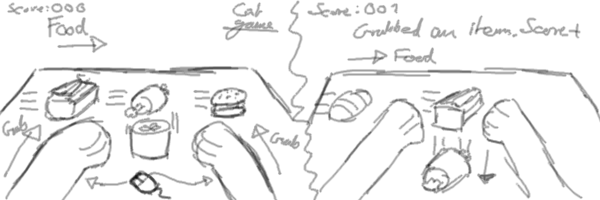
\includegraphics[width=\textwidth]{img/storyboard/original_1.png}
                \caption{Storyboard: Grabbing items as they go past on a conveyor belt}
                \label{fig:original1}
        \end{subfigure}

%
        %add desired spacing between images, e. g. ~, \quad, \qquad etc.
          %(or a blank line to force the subfigure onto a new line)
        \begin{subfigure}[b]{0.8\textwidth}
                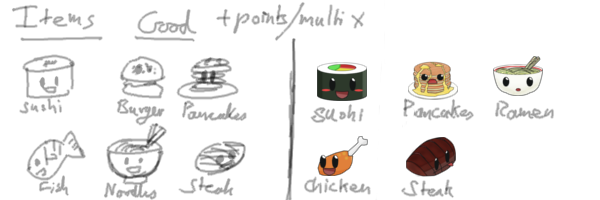
\includegraphics[width=\textwidth]{img/storyboard/original_foods.png}
                \caption{The concept for the 'good' food items and their eventual finished designs}
                \label{fig:originalfoods}
        \end{subfigure}
        \caption{Original concepts and storyboards}\label{fig:concepts1}
\end{figure}

I developed this further to where the user could click as fast as they wanted, but had to use alternate clicks (Left to Right) to collect items. A consecutive click of a single button (Left to Left/Right to Right) would result in knocking an item away and losing a life.This presented issues with animating as fast as the clicks and didn't really seem engaging.

\begin{figure}[H]
        \centering
        \begin{subfigure}[b]{0.8\textwidth}
                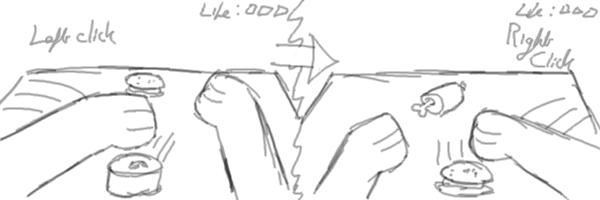
\includegraphics[width=\textwidth]{img/storyboard/original_2.png}
                \caption{Storyboard: Alternating mouse clicks grabs food with each paw.}
                \label{fig:original2}
        \end{subfigure}

%
        %add desired spacing between images, e. g. ~, \quad, \qquad etc.
          %(or a blank line to force the subfigure onto a new line)
        \begin{subfigure}[b]{0.8\textwidth}
                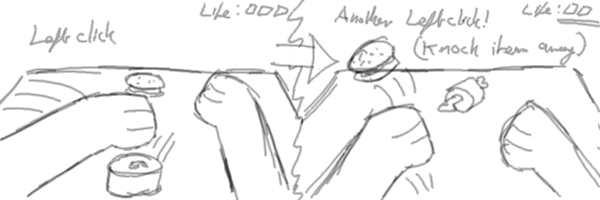
\includegraphics[width=\textwidth]{img/storyboard/original_3.png}
                \caption{Storyboard: Clicking the same button twice in a row knocks items off the table}
                \label{fig:original3}
        \end{subfigure}
        \caption{Concepts: Mouse clicks and their results}\label{fig:concepts2}
\end{figure}

My resulting idea was to combine both of my previous ideas, plus a couple of 'wildcards': Bad items and the 'Watcher'.
\begin{figure}[H]
  \centering
    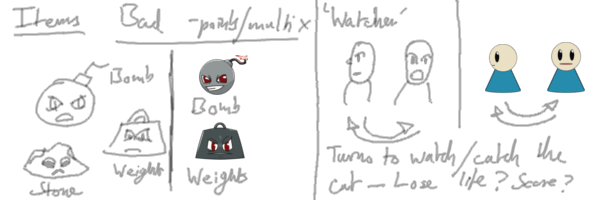
\includegraphics[width=0.8\textwidth]{img/storyboard/original_bad}
  \caption{Bad items and the 'Watcher'.}
\end{figure}
 Both bad items and the Watcher could remove some of the players score/multiplier/lives, with the bad items needing to be 'knocked' away while the Watcher forces the player to be aware of the game as they played. 
\begin{figure}[H]
  \centering
    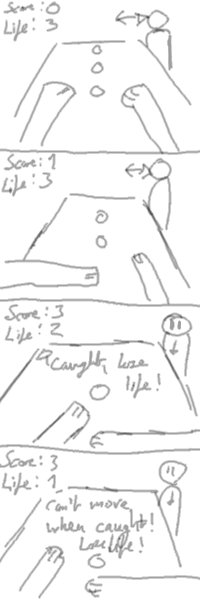
\includegraphics[width=0.3\textwidth]{img/storyboard/original_watcher.png}
  \caption{Storyboard: A player caught by the 'Watcher', then trying to move again.}
\end{figure}

My final game has a player use left and right click alternately to 'eat' good items for points, and use them consecutively to knock bad items away. They must also be mindful of a 'Watcher' that will randomly stare at them. If they click to move when the Watcher is looking, they lose a life.

The player starts with 5 lives. Every 15 good items eaten doubles a score multiplier, but also makes the Watcher stare more frequently. Any failure (knock a good item, eat a bad item, get caught), resets the multiplier. Eating a bad item reduces the players score and the game ends when all lives are lost.

These aspects make the game dynamic, with moments where the player must pause and wait for the watcher, or get caught outright by them when quickly clicking. I feel my resulting game fulfills my purpose of a simple game, yet tricky enough to make people want to play more and challenge their friends.

%----------------------------------------------------------------------------------------
%	TECHNICAL OVERVIEW
%----------------------------------------------------------------------------------------

\section{Technical Overview}
The application is written in HTML5, using the \begin{math}<canvas>\end{math} element and JavaScript. There is no server side script, so the game runs on a users machine, saving load on my webpage's server. I used the JQuery library to detect the particular mouse button being clicked and disable the appearance of the menu on a right-click.

There are other technologies I could have used (e.g. Flash). I decided to stick with JavaScript though as it is relatively well supported by most modern browsers and well documented (with help accessible for it over the Internet, i.e. W3Schools\cite{w3c}).

JavaScript is relatively easy to program with, coming from using languages such as C and Java previously, and can be programmed functionally and made to seem like an Object Oriented language. Being able to control the flow of the data and treat it as a language with 'objects' made coding simple, and easy to control the elements of the game on the canvas and in the data.

%----------------------------------------------------------------------------------------
%	SOFTWARE TESTING
%----------------------------------------------------------------------------------------

\section{Software Testing}
I tested my game in Google Chrome, Mozilla's Firefox and Internet Explorer Edge browsers. The game functions similarly on each, with little to no discrepancies. As can be seen below, the game looks very similar in each browser and, when playing the game, seems to run the same too.

\begin{figure}[H]
        \centering
        \begin{subfigure}[b]{0.4\textwidth}
                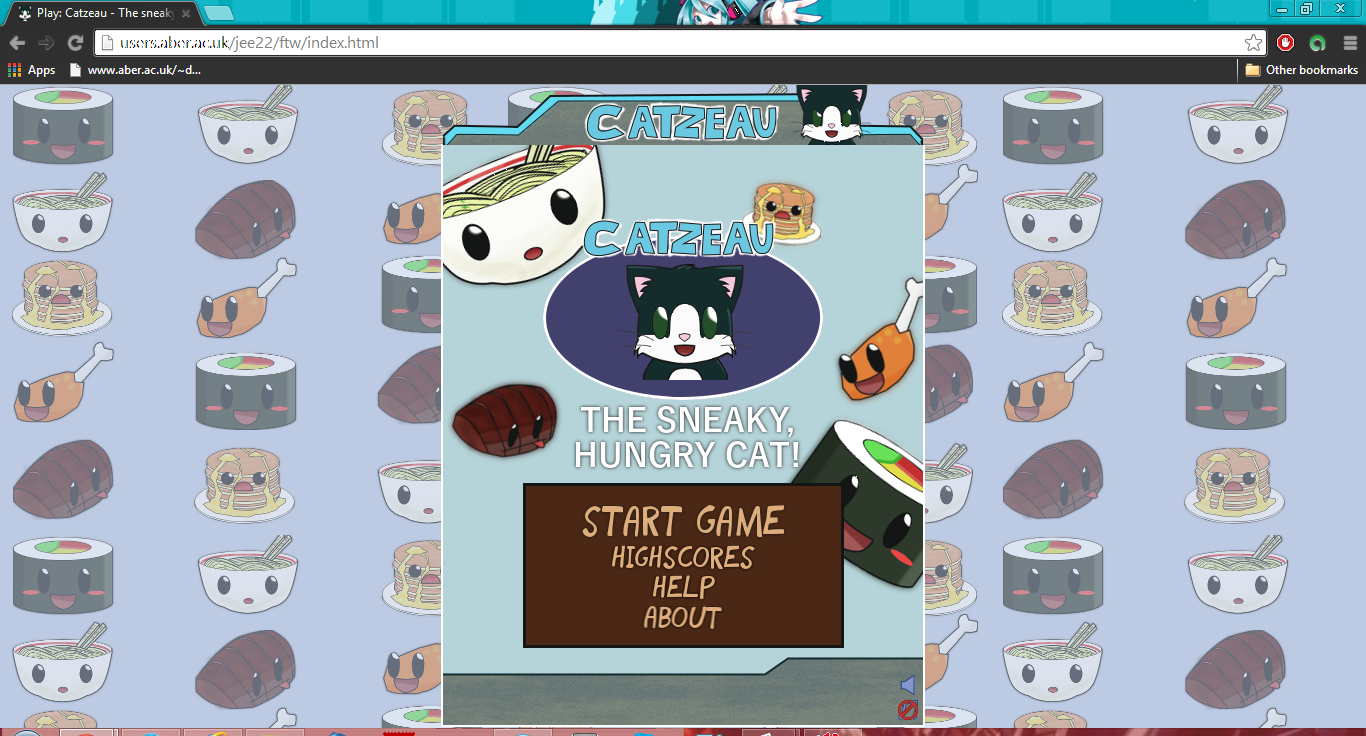
\includegraphics[width=\textwidth]{img/testing/chrome_start.png}
                \caption{The start menu in Chrome}
                \label{fig:chromestart}
        \end{subfigure}
        ~%add desired spacing between images, e. g. ~, \quad, \qquad etc.
          %(or a blank line to force the subfigure onto a new line)
        \begin{subfigure}[b]{0.4\textwidth}
                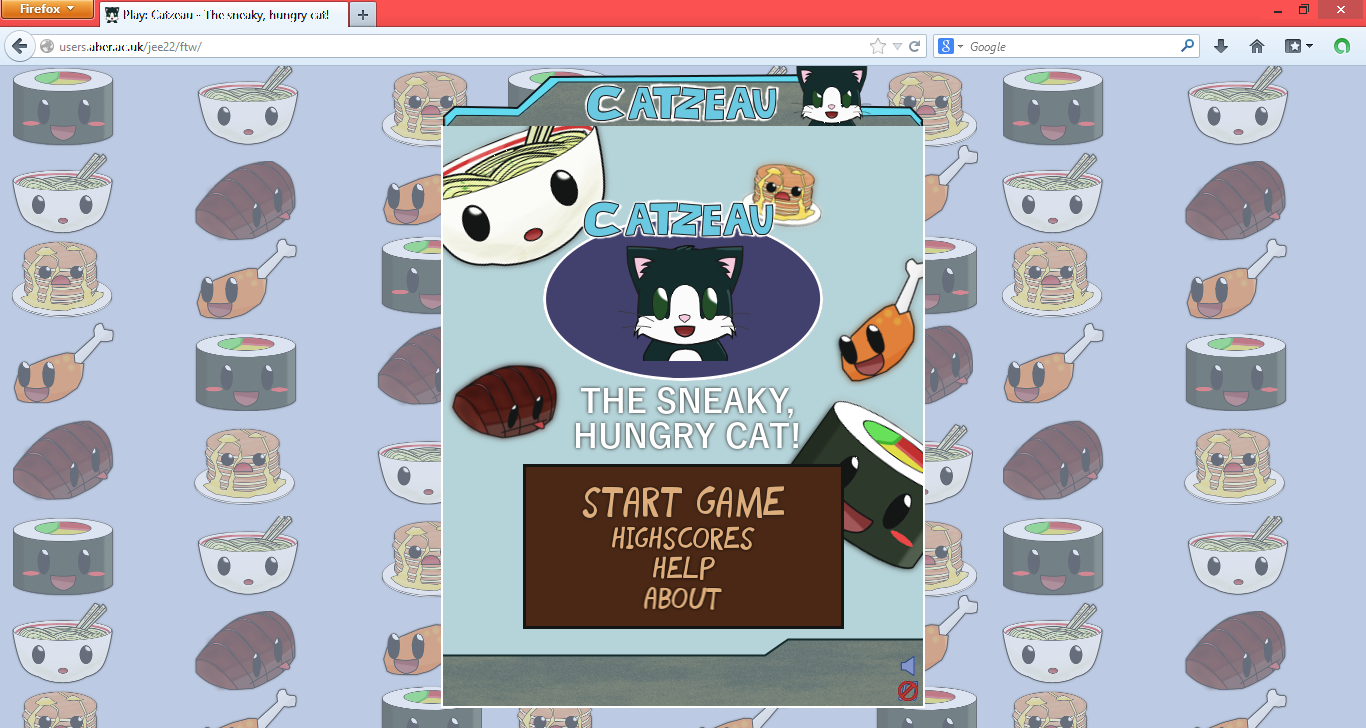
\includegraphics[width=\textwidth]{img/testing/ff_start.png}
                \caption{The start menu in Firefox}
                \label{fig:firefoxstart}
        \end{subfigure}
	~
        \begin{subfigure}[b]{0.4\textwidth}
                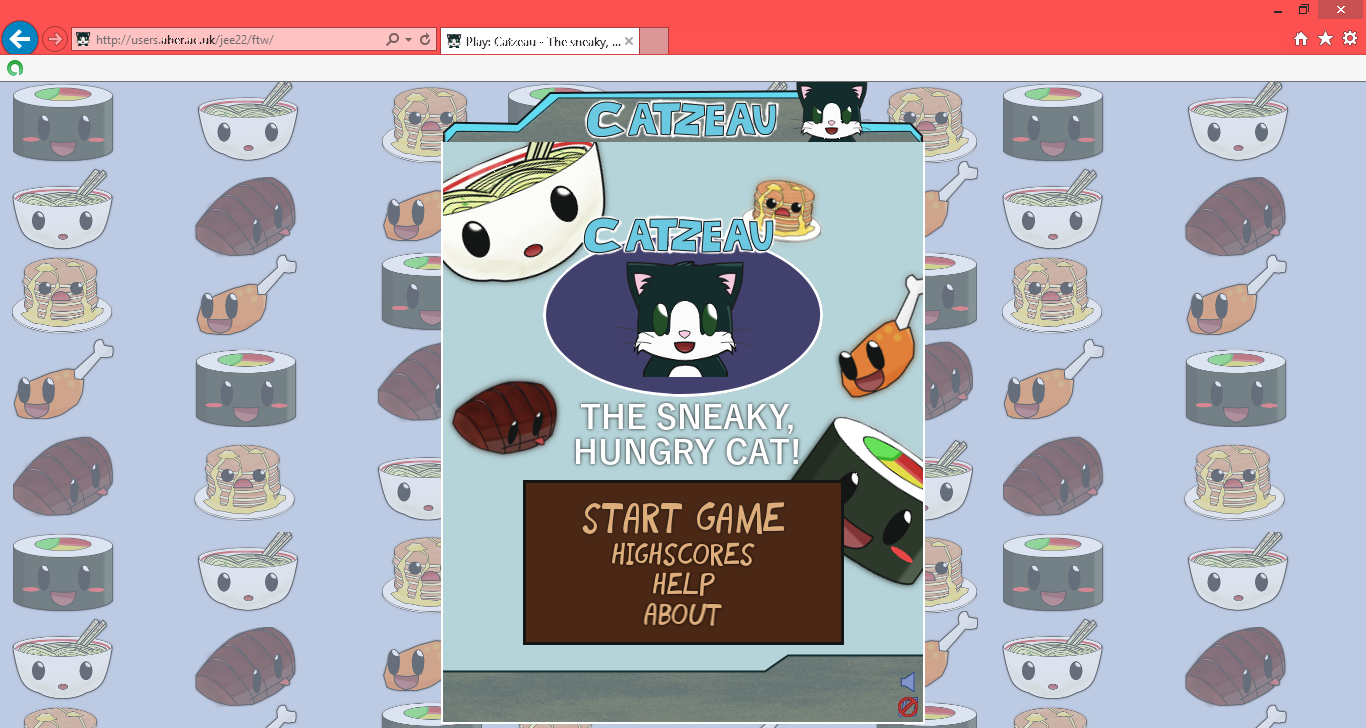
\includegraphics[width=\textwidth]{img/testing/ie_start.png}
                \caption{The start menu in Internet Explorer Edge}
                \label{fig:iestart}
        \end{subfigure}
\end{figure}

The game runs on a mobile device, but since the game uses two mouse buttons on a single screen, it only responds to the left click. I could program the application to accept taps on the two sides of the screen in replacement, but I felt this was out of the scope of the assignment, and could be a future revision.

        \begin{figure}[H]
	\centering
                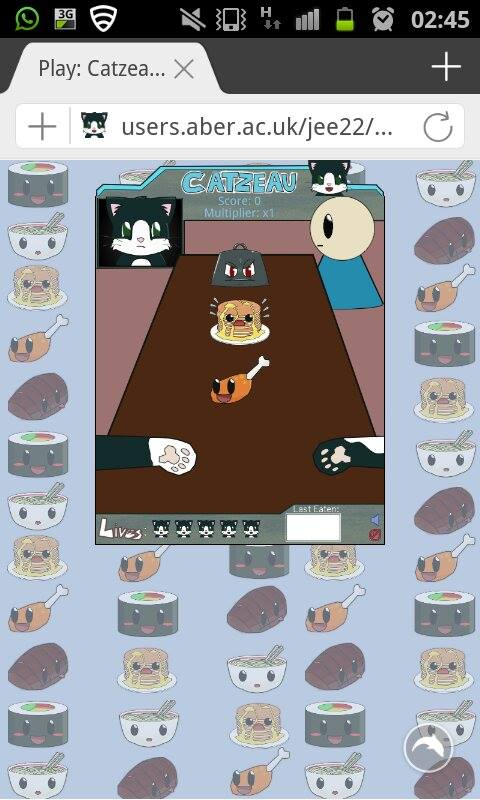
\includegraphics[width=0.3\textwidth]{img/testing/phone.jpg}
                \caption{The gameplay using the Dolphin browser on a Samsung phone running Android 2.3}
                \label{fig:phone}
        \end{figure}

There were a few differences between browsers that needed to be accommodated for during my testing, such as IE not pausing the sound effects after being played, and some issues loading localstorage in Firefox. These tended to be minor and did not cause any current standing issues.

%----------------------------------------------------------------------------------------
%	REFLECTIONS & FUTURE WORK
%----------------------------------------------------------------------------------------

\section{Reflections \& Future Work}
There are multiple ways I would improve the game. First, I'd implement a working mobile version. In terms of gameplay, I would add more varieties of items, and improve the graphics and AI of the 'Watcher'. I also wanted to implement a 'bonus mode', where a particular item could be consumed to 'dubstepify' the game.

Following this would be different difficulties, and modes where there is no Watcher/only good items. I even considered rewards for high scores, like different aesthetic affects or permanent toggle-able power ups. I'd also add a global high scores table, with social integration for posting scores to Facebook/Twitter, boosting the competitive side.

These are all things I'd implement were I to continue working on this project and to be considered as a marketable product, especially as it seems to fit in the vein of casual mobile gaming. Right now it is not ready to generate money. I have learned a great deal from this game, and know I will continue to create HTML5 applications in the future, utilizing what I have learned during it's creation. 

%----------------------------------------------------------------------------------------
\clearpage

%----------------------------------------------------------------------------------------
%	REFERENCES
%----------------------------------------------------------------------------------------

\begin{thebibliography}{1}

\bibitem{assignment} H. Dee, "CS25210 Coursework 2014: An HTML5 Canvas game with animated sprites.", CS25210 Assessed Assignment 2013-2014, February 2014

\bibitem{w3c} W3schools.com (Accessed 18/04/2014) JavaScript Tutorial [Online]. Available: http://www.w3schools.com/js/



\end{thebibliography}


\end{document}


